\documentclass[../main]{subfiles}

% Chapter 2: a results chapter adapted from the author's own papers. It
% shows the whole-chapter disclaimer, a multi-panel figure, a table, the
% \sectionclose that ends each section and the closing "Summary: ..." section.

\begin{document}
% In a standalone build, start the chapter counter where it would be.
\ifSubfilesClassLoaded{\setcounter{chapter}{1}}{}

\chapter{Main Results}
\label{ch:ch2}
% An epigraph in Greek with its English translation: \foreignlanguage for
% the Greek lines, which use the polytonic Greek font of preamble/fonts.tex.
\begin{chquote}
\foreignlanguage{greek}{παράδειγμα ἐπιγραφῆς} \\
\vspace{1em}
An example of an epigraph, \\
followed by its translation. \\
\bigskip
-- Author, \textit{Work} \foreignlanguage{greek}{α}
\end{chquote}

\begin{chabstract}
This chapter presents the main results of the thesis.
It shows a multi-panel figure, a table and the summary section that closes every results chapter.
\end{chabstract}

% A chapter that reuses material from published papers says so here,
% right after the chapter abstract. Do not re-cite those papers sentence by
% sentence in the chapter: the disclaimer covers the attribution.
\begin{disclaimer}
This chapter is an adaptation and extension of Refs.~\cite{Doe:PRB24, Roe:PRL25, Doe:SP25}.
\end{disclaimer}

\clearpage
The lead-in links the chapter to the previous ones, for instance to Section~\ref{sec:equations} of Chapter~\ref{ch:ch1}.
Acronyms are expanded again at their first occurrence in each chapter, as \acrfull{ldos}, and are short afterwards, \acrshort{ldos}.
\lipsum[1][1-5]
In Section~\ref{sec:model} we introduce the model, and in Section~\ref{sec:results} we present the results, summarized in Section~\ref{sec:ch2_summary}.

% ── Section ──────────────────────────────────────────────────
\section{The model}
\label{sec:model}
\lipsum[2][1-4]

\subsection{Hamiltonian}
\label{sec:hamiltonian}
We start from the Hamiltonian of Eq.~\eqref{eq:example} and add a term,
\begin{equation}
    \label{eq:ch2_hamiltonian}
    \tilde{H} = H + V_\text{Z}\sigma_z,
\end{equation}
where $V_\text{Z}$ is the Zeeman energy.
\lipsum[3][1-5]

\subsection{Parameters}
\label{sec:parameters}
Table~\ref{tab:parameters} collects the parameters used in this chapter.
Physical quantities with units use \verb|siunitx|, as in \SI{0.2}{\milli\electronvolt} or \SI{100}{\nano\meter}.

% Tables: booktabs rules, caption above the table, same bold-summary style
% as figure captions.
\begin{table}[hbtp]
    \centering
    \caption[Parameters of the mock-up model]{\textbf{Parameters of the mock-up model.}
    Values used in all the figures of this chapter unless stated otherwise.
    }
    \label{tab:parameters}
    \begin{tabular}{@{}llr@{}}
        \toprule
        Parameter & Symbol & Value \\
        \midrule
        Effective mass & $m^*$ & $0.023m_e$ \\
        Chemical potential & $\mu$ & \SI{1}{\milli\electronvolt} \\
        Pairing & $\Delta$ & \SI{0.2}{\milli\electronvolt} \\
        Spin-orbit coupling & $\alpha$ & \SI{20}{\milli\electronvolt\nano\meter} \\
        Radius & $R$ & \SI{70}{\nano\meter} \\
        \bottomrule
    \end{tabular}
\end{table}

\lipsum[4][1-5]

% Every section of a results chapter ends with a synthesis after \sectionclose.
\sectionclose
This paragraph summarizes the section on the model.
\lipsum[5][1-2]

% ── Section ──────────────────────────────────────────────────
\section{Results}
\label{sec:results}
\lipsum[6][1-3]

\subsection{A multi-panel figure}
\label{sec:multipanel}
Figure~\ref{fig:mock_panels} shows the three panels of a full-width figure.
In the text, panels are referred to as Fig.~\ref{fig:mock_panels}(a) or Figs.~\ref{fig:mock_panels}(b) and~\ref{fig:mock_panels}(c).
The \acrshort{ldos} of panel (b) peaks at the center.

\begin{figure}[hbtp]
    \centering
    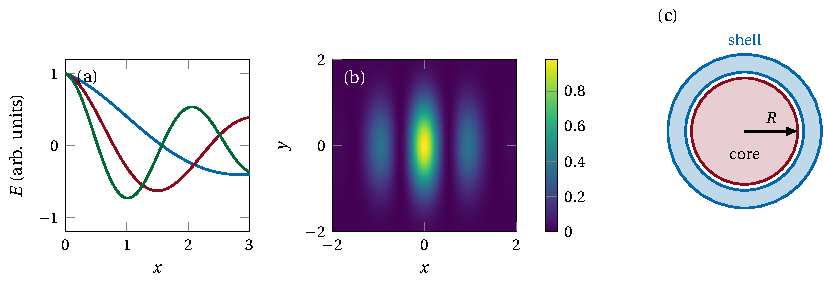
\includegraphics{figures/mock_panels.pdf}
    \caption[A multi-panel mock-up figure]{\textbf{A multi-panel mock-up figure.}
    A bold one-line summary comes first, then one block per panel.
    (a) Three damped oscillations, in arbitrary units.
    Each sentence of a panel sits on its own source line.
    (b) Mock \acrfull{ldos} as a function of the position $(x, y)$.
    (c) Schematic of a core (red) inside a shell (blue), with radius $R$.
    }
    \label{fig:mock_panels}
\end{figure}

\lipsum[7][1-6]

\subsection{Comparison with other works}
\label{sec:comparison}
Other publications of the author that are not part of the thesis can be cited too, and keep their N label~\cite{Lee:PRB23, Kowalski:PRB26}.
A paper with an erratum is cited once, and the erratum is printed in the same bibliography item~\cite{Smith:PRL20}.
Author lists longer than six names are truncated to two and ``et al.'', and journals without a short-name mapping keep their full name~\cite{Garcia:NP22}.
Preprints~\cite{Lee:a23}, book chapters~\cite{Roe:18} and conference proceedings~\cite{Kowalski:17} have their own formats.
\lipsum[8][1-5]

\sectionclose
This paragraph summarizes the section on the results.
\lipsum[9][1-2]

% ── Summary section, titled "Summary: ..." in every chapter ─
\section{Summary: main results}
\label{sec:ch2_summary}
The summary section closes the chapter and connects it to the next one.
\lipsum[10-11]
These results set the stage for the conclusions of Chapter~\ref{ch:ch3}.

\ifSubfilesClassLoaded{%
\newrefcontext[labelprefix=]
\printbibliography
}{}
\end{document}
